%========================================================================
% Modelo para elaboracao de textos academicos: TCC, dissertacoes e teses
% Elaborado pelo GISIS - Grupo de Imageamento Sismico e Inversao Sismica.
%========================================================================
\chapter{Resultados}
\label{ch:resultados}


\begin{figure}[H]
	\centering
	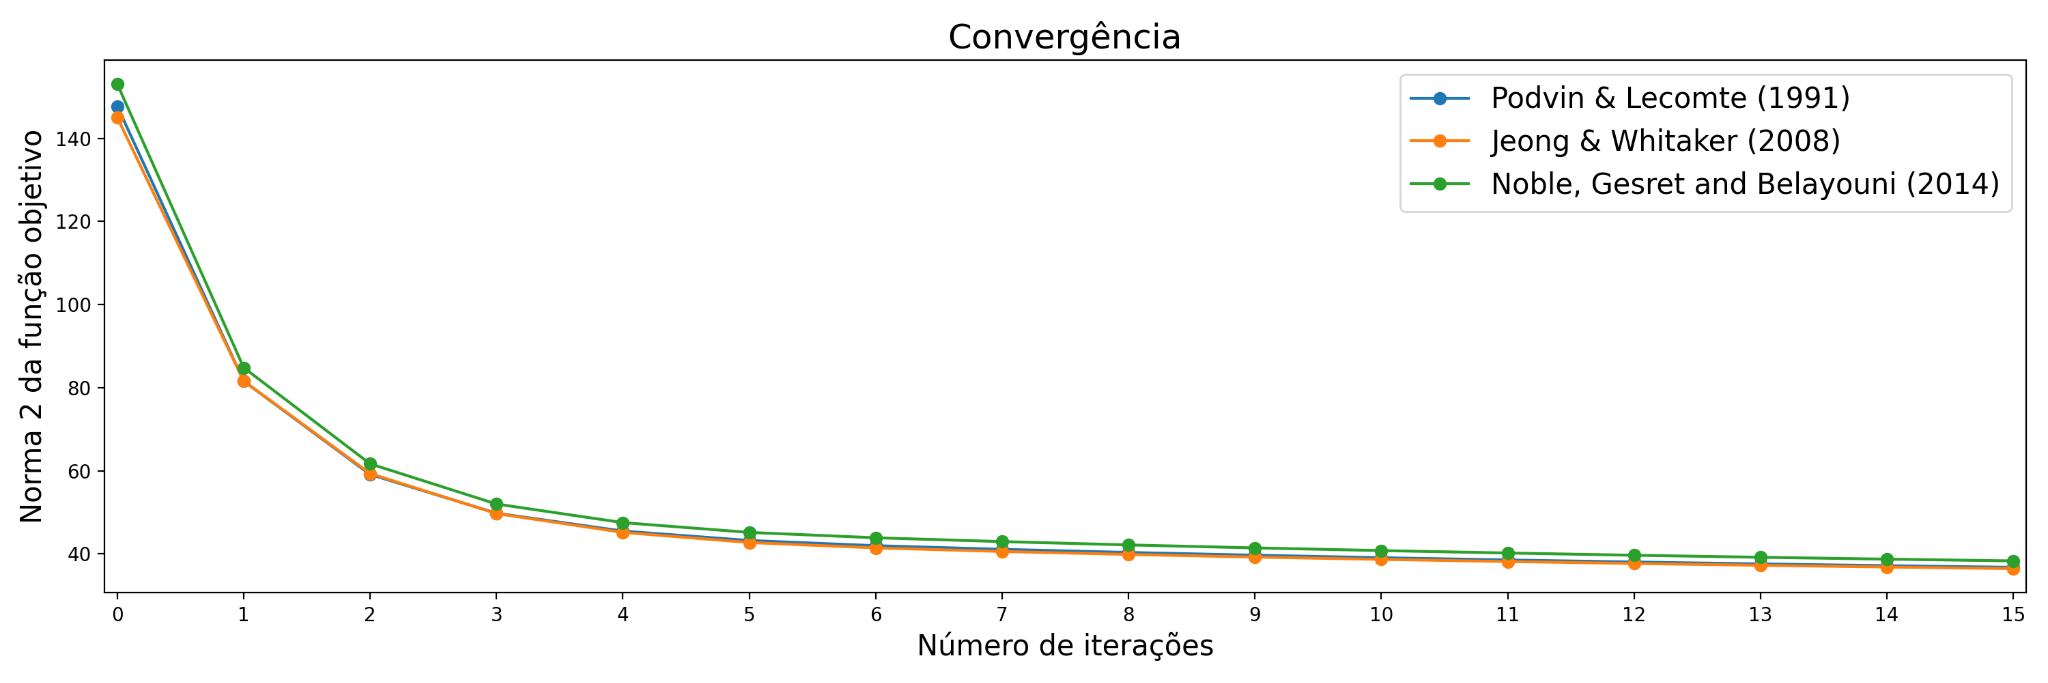
\includegraphics[width=16cm,height=6cm]{Imgs/Resultados/convergencia.png}
	\caption{caption}
	\label{fig:}	
\end{figure}



\section{Inversão com malha esparsa}



\begin{figure}[H]
	\centering
	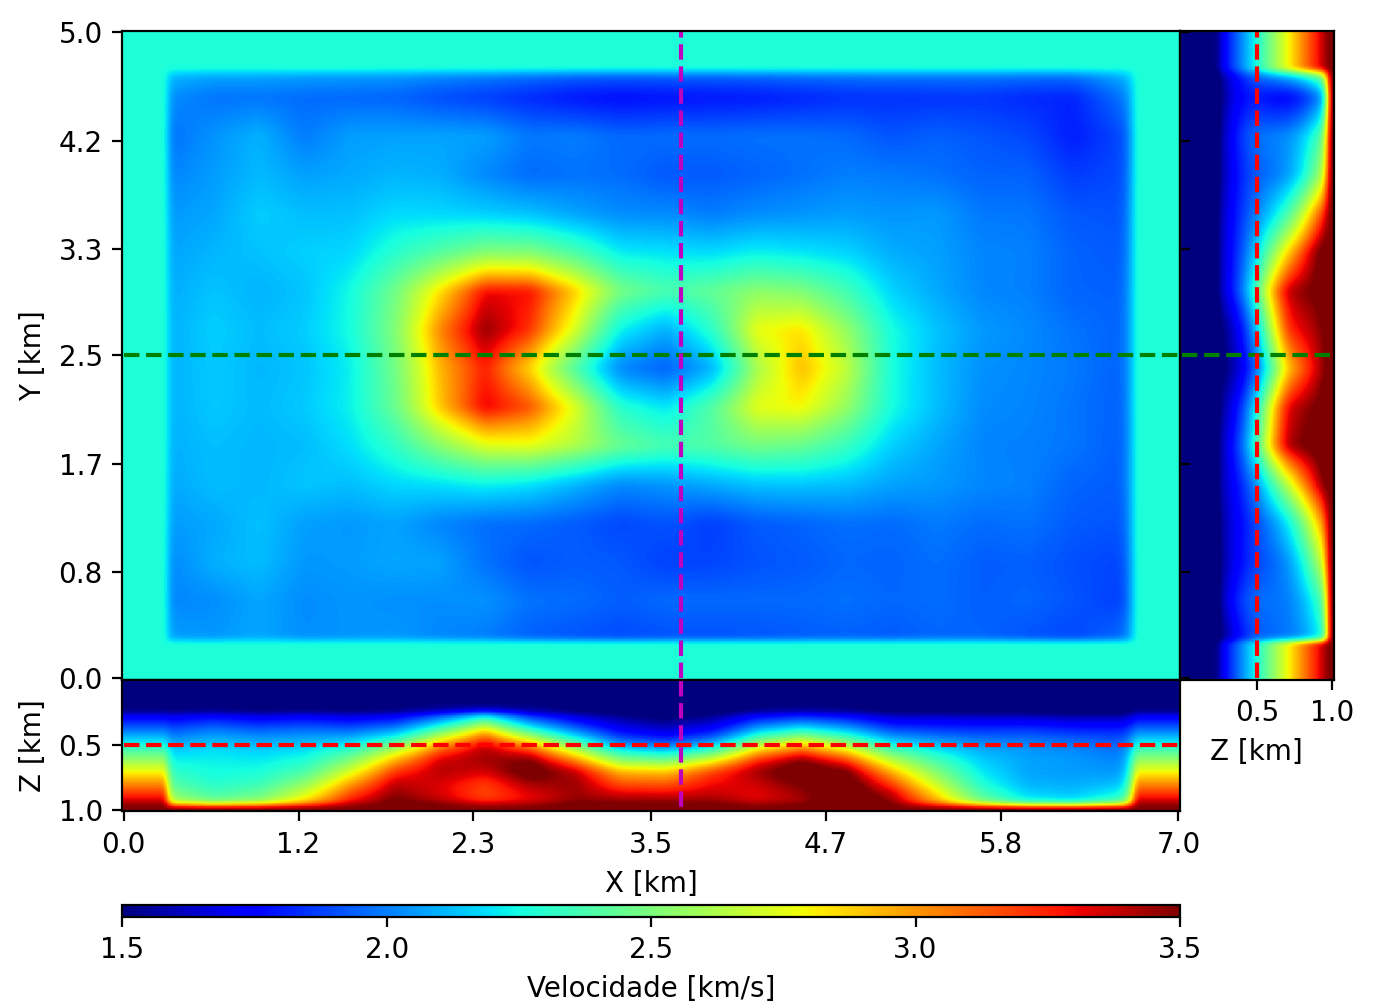
\includegraphics[width=12cm,height=9cm]{Imgs/Resultados/pod_sparse.png}
	\caption{caption}
	\label{fig:}	
\end{figure}


\begin{figure}[H]
	\centering
	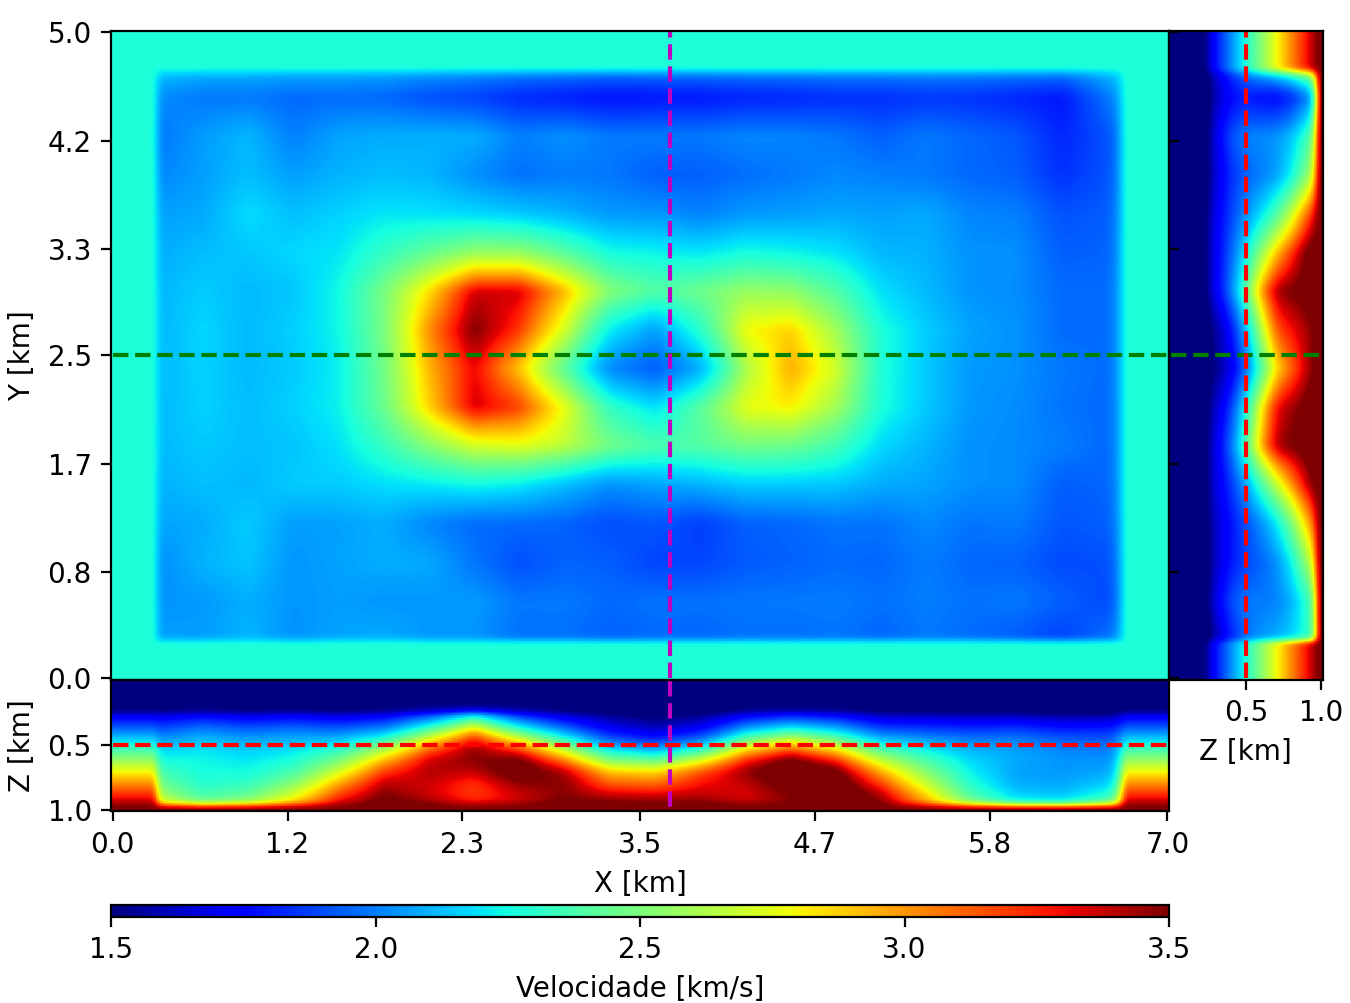
\includegraphics[width=12cm,height=9cm]{Imgs/Resultados/fim_sparse.png}
	\caption{caption}
	\label{fig:}	
\end{figure}


\begin{figure}[H]
	\centering
	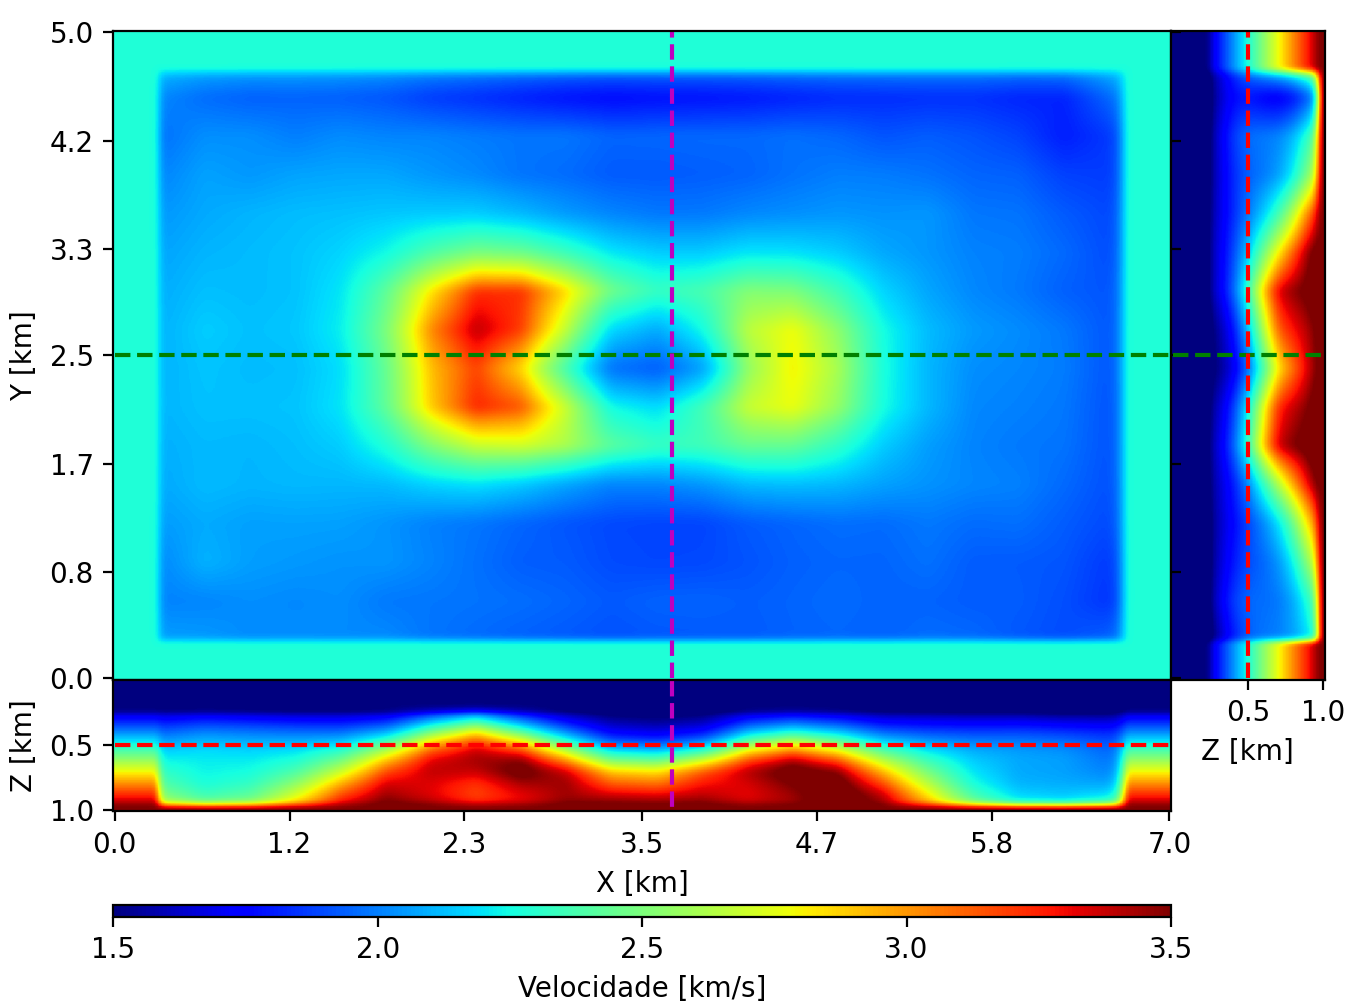
\includegraphics[width=12cm,height=9cm]{Imgs/Resultados/fsm_sparse.png}
	\caption{caption}
	\label{fig:}	
\end{figure}


\section{Inversão com malha refinada}

\begin{figure}[H]
	\centering
	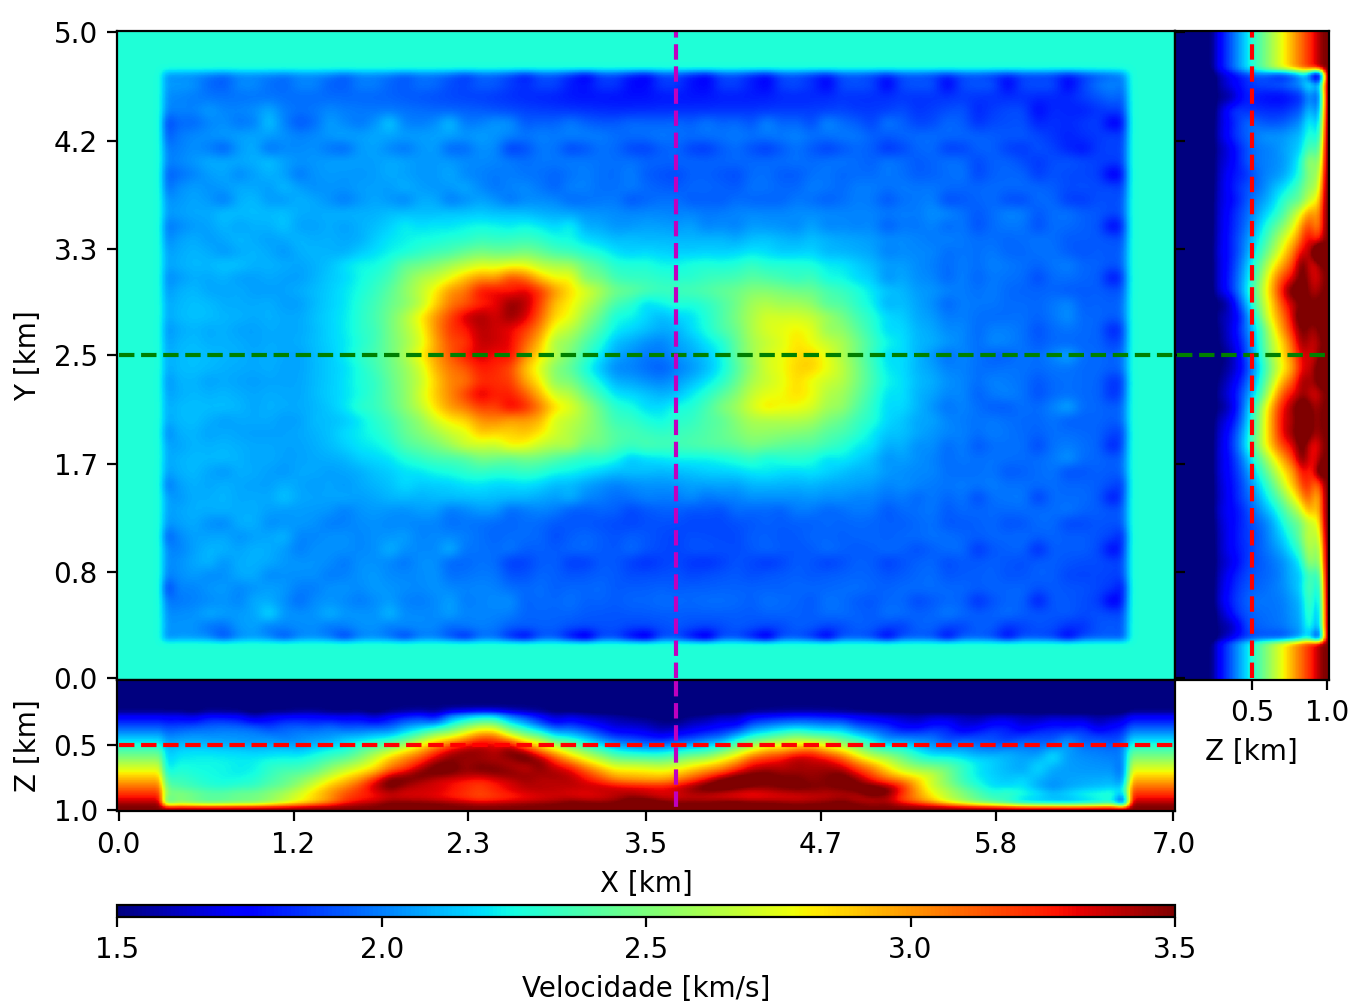
\includegraphics[width=12cm,height=9cm]{Imgs/Resultados/pod_refined.png}
	\caption{caption}
	\label{fig:}	
\end{figure}


\begin{figure}[H]
	\centering
	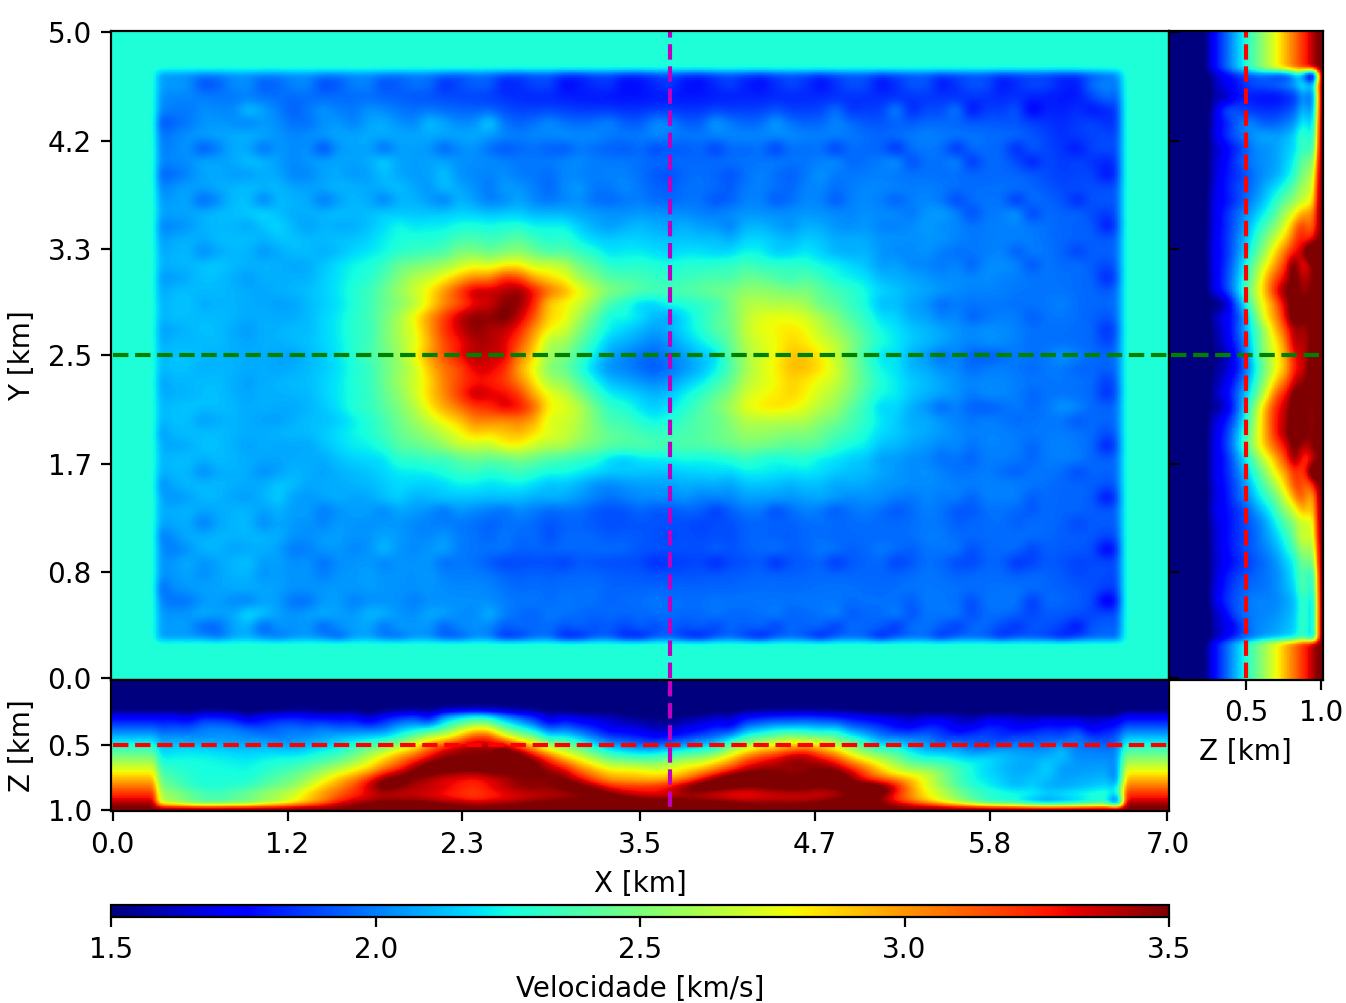
\includegraphics[width=12cm,height=9cm]{Imgs/Resultados/fim_refined.png}
	\caption{caption}
	\label{fig:}	
\end{figure}


\begin{figure}[H]
	\centering
	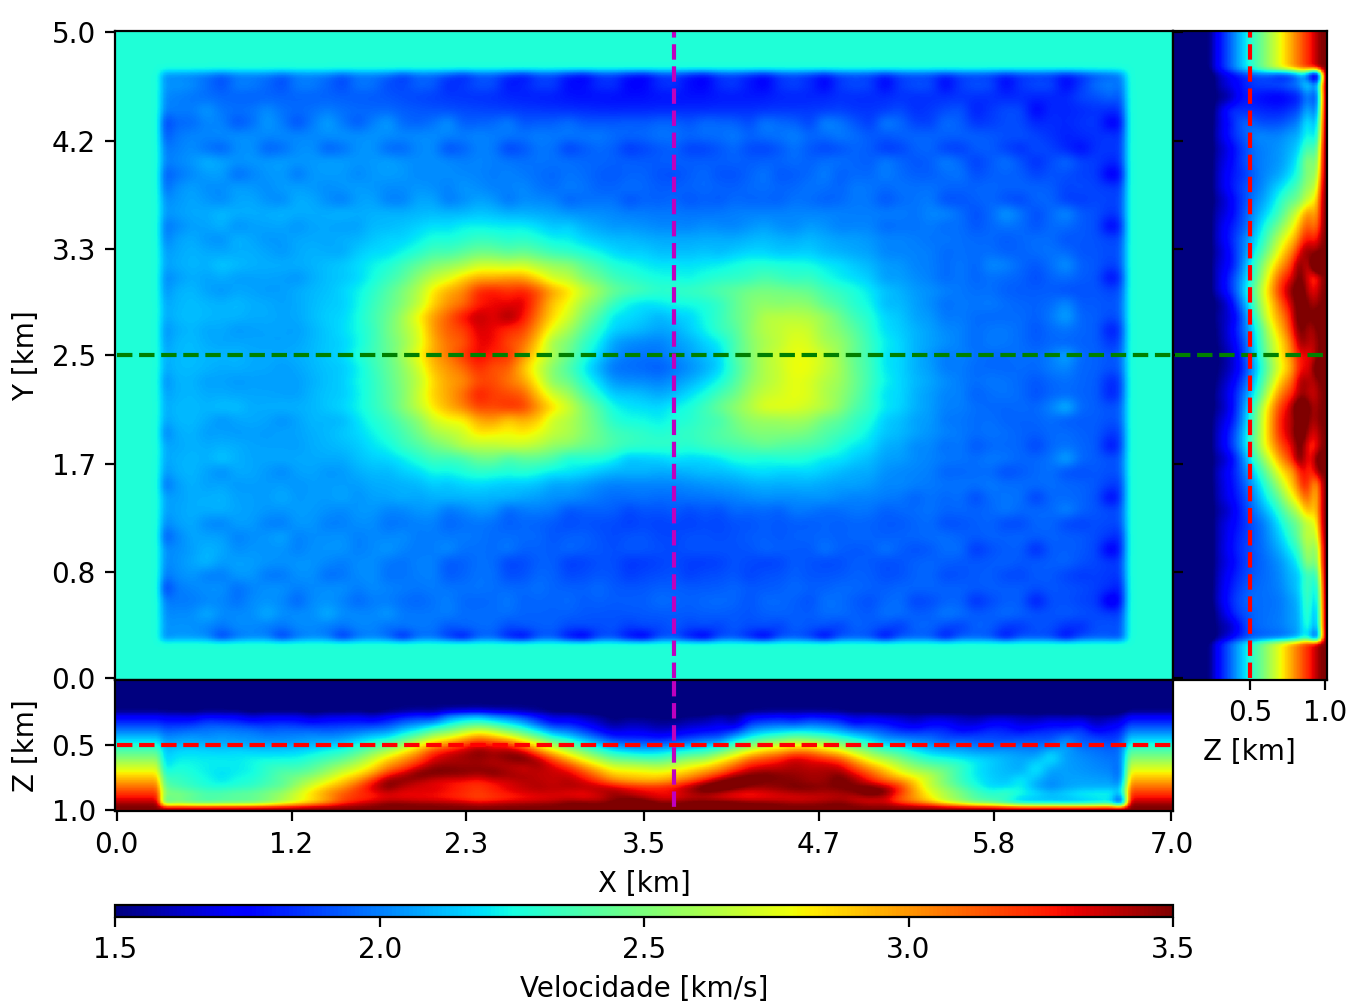
\includegraphics[width=12cm,height=9cm]{Imgs/Resultados/fsm_refined.png}
	\caption{caption}
	\label{fig:}	
\end{figure}





